\chapter{Setting up PR2 in your lab}
\section{Taking PR2 out of the crate}
The PR2 will arrive in a large crate, it is important to place the crate in an
open area with at least 10 feet of space infront of the the panel labeled {\bf
  FRONT}, Figure~\ref{fig:crate_space}, and 5 feet on all other
sides (including behind the crate).

\begin{figure}[h!]
\centering
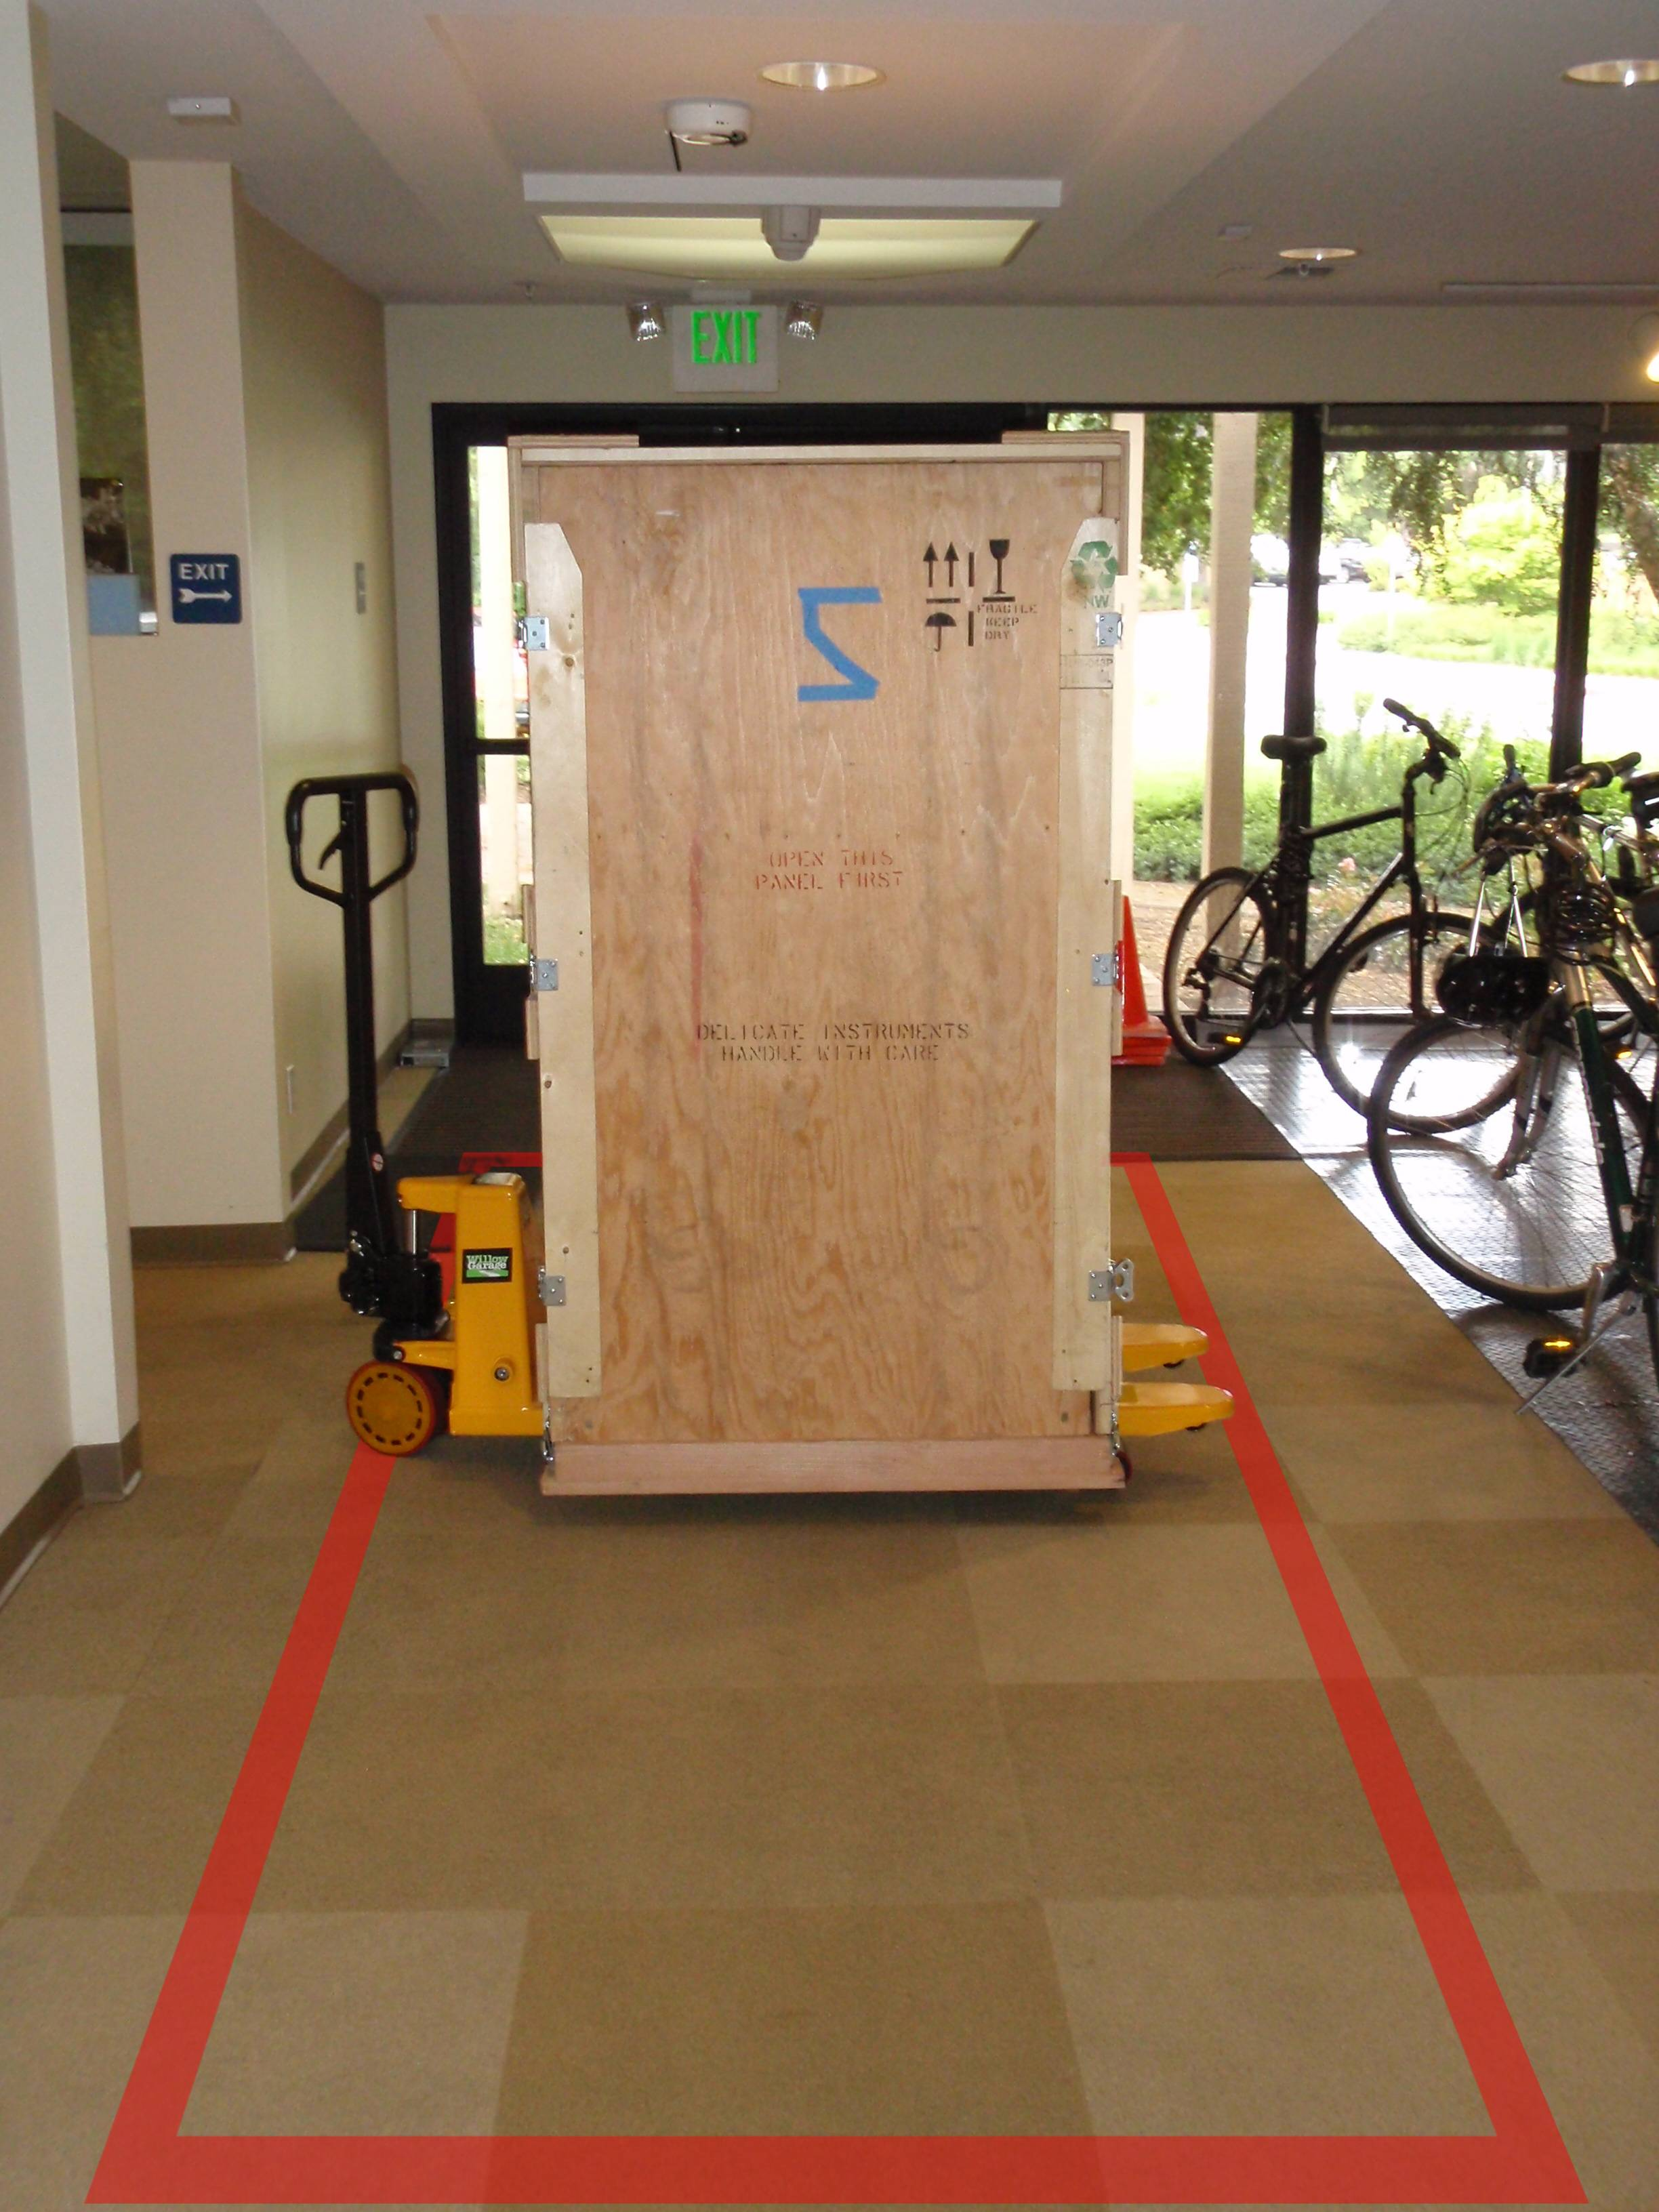
\includegraphics[width=150px]{crate_area_lowres.jpg}
\caption{The space required to uncrate a PR2.}
\label{fig:crate_space}
\end{figure}

Now that there is adequate room around the crate, begin opening the crate by
unlatching the metal latches around the panel labeled {\bf OPEN THIS PANEL
  FIRST}, Figure~\ref{fig:unlatch}. Lift the latch up then rotate the latch
handle counter-clockwise until the hook is extended and no longer
engaged. Finally push the hook outwards to disengage the latch.

\begin{figure}[h]
\centering
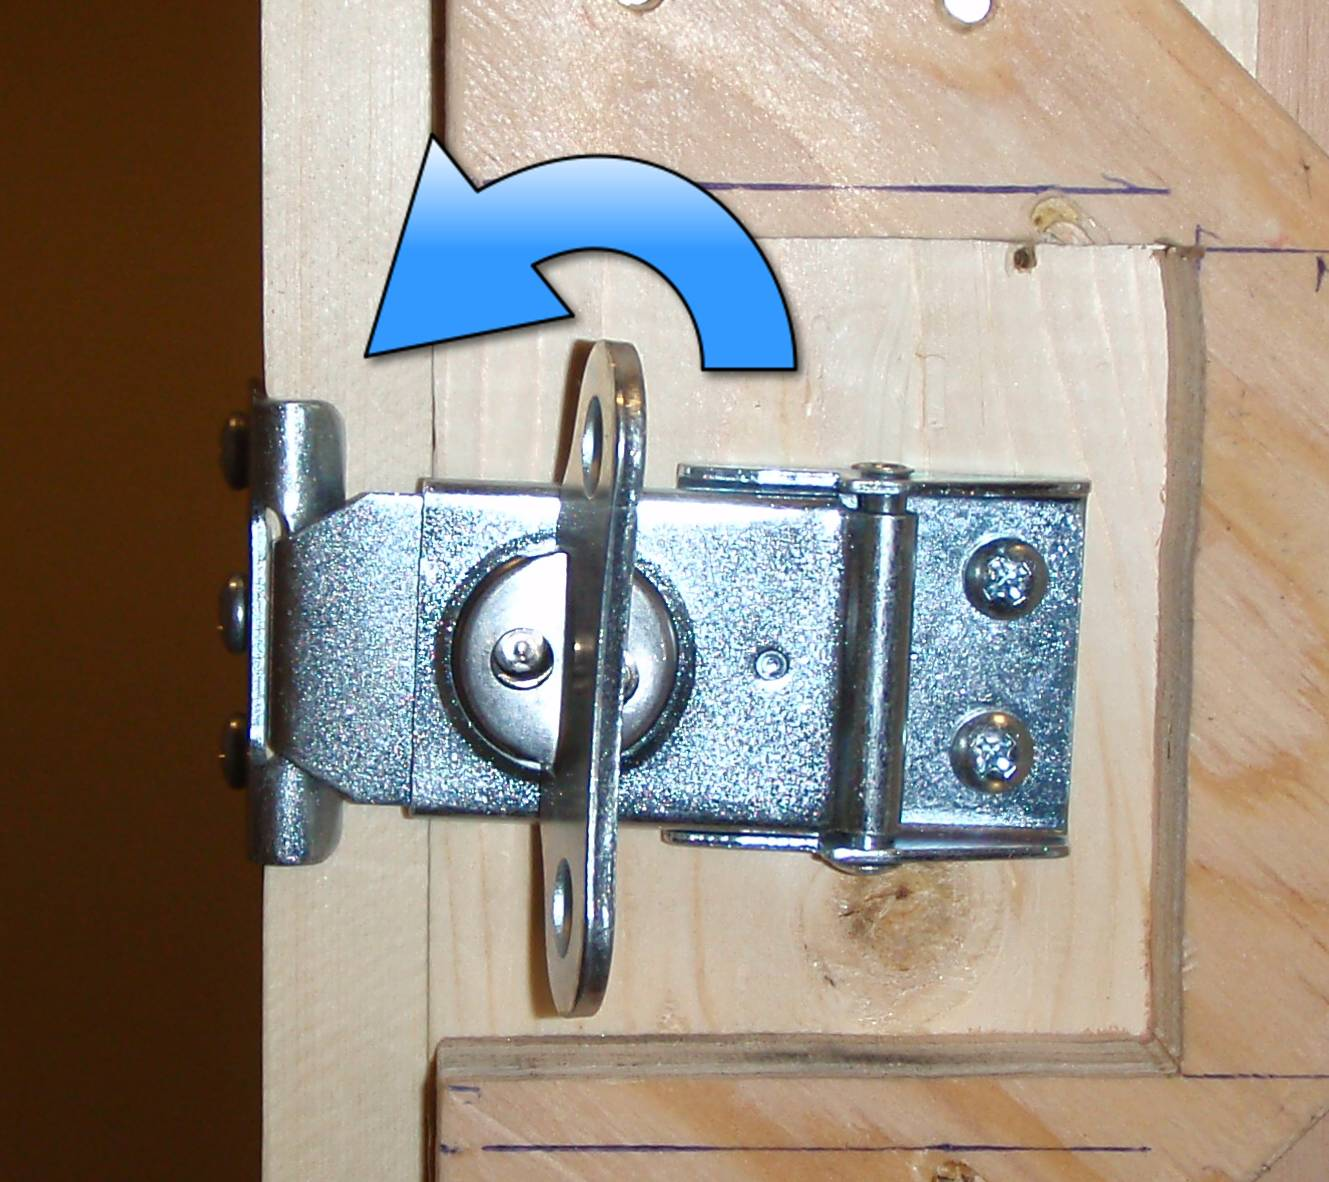
\includegraphics[width=150px]{unlatching_lowres.jpg}
\caption{PR2 crate twist latch.}
\label{fig:unlatch}
\end{figure}

Unlatch the six latches on the front panel and set the panel aside for use
later. Inside the crate is a vaccuum sealed PR2, Figure~\ref{fig:sealPR2},
unlatch and remove the two boards holding the head in place. After the boards
are removed, unlatch all of the latches aroung the bottom of the crate. Make
sure that all of the latch hooks are pushed down and out of the way.

\begin{figure}[h]
\centering
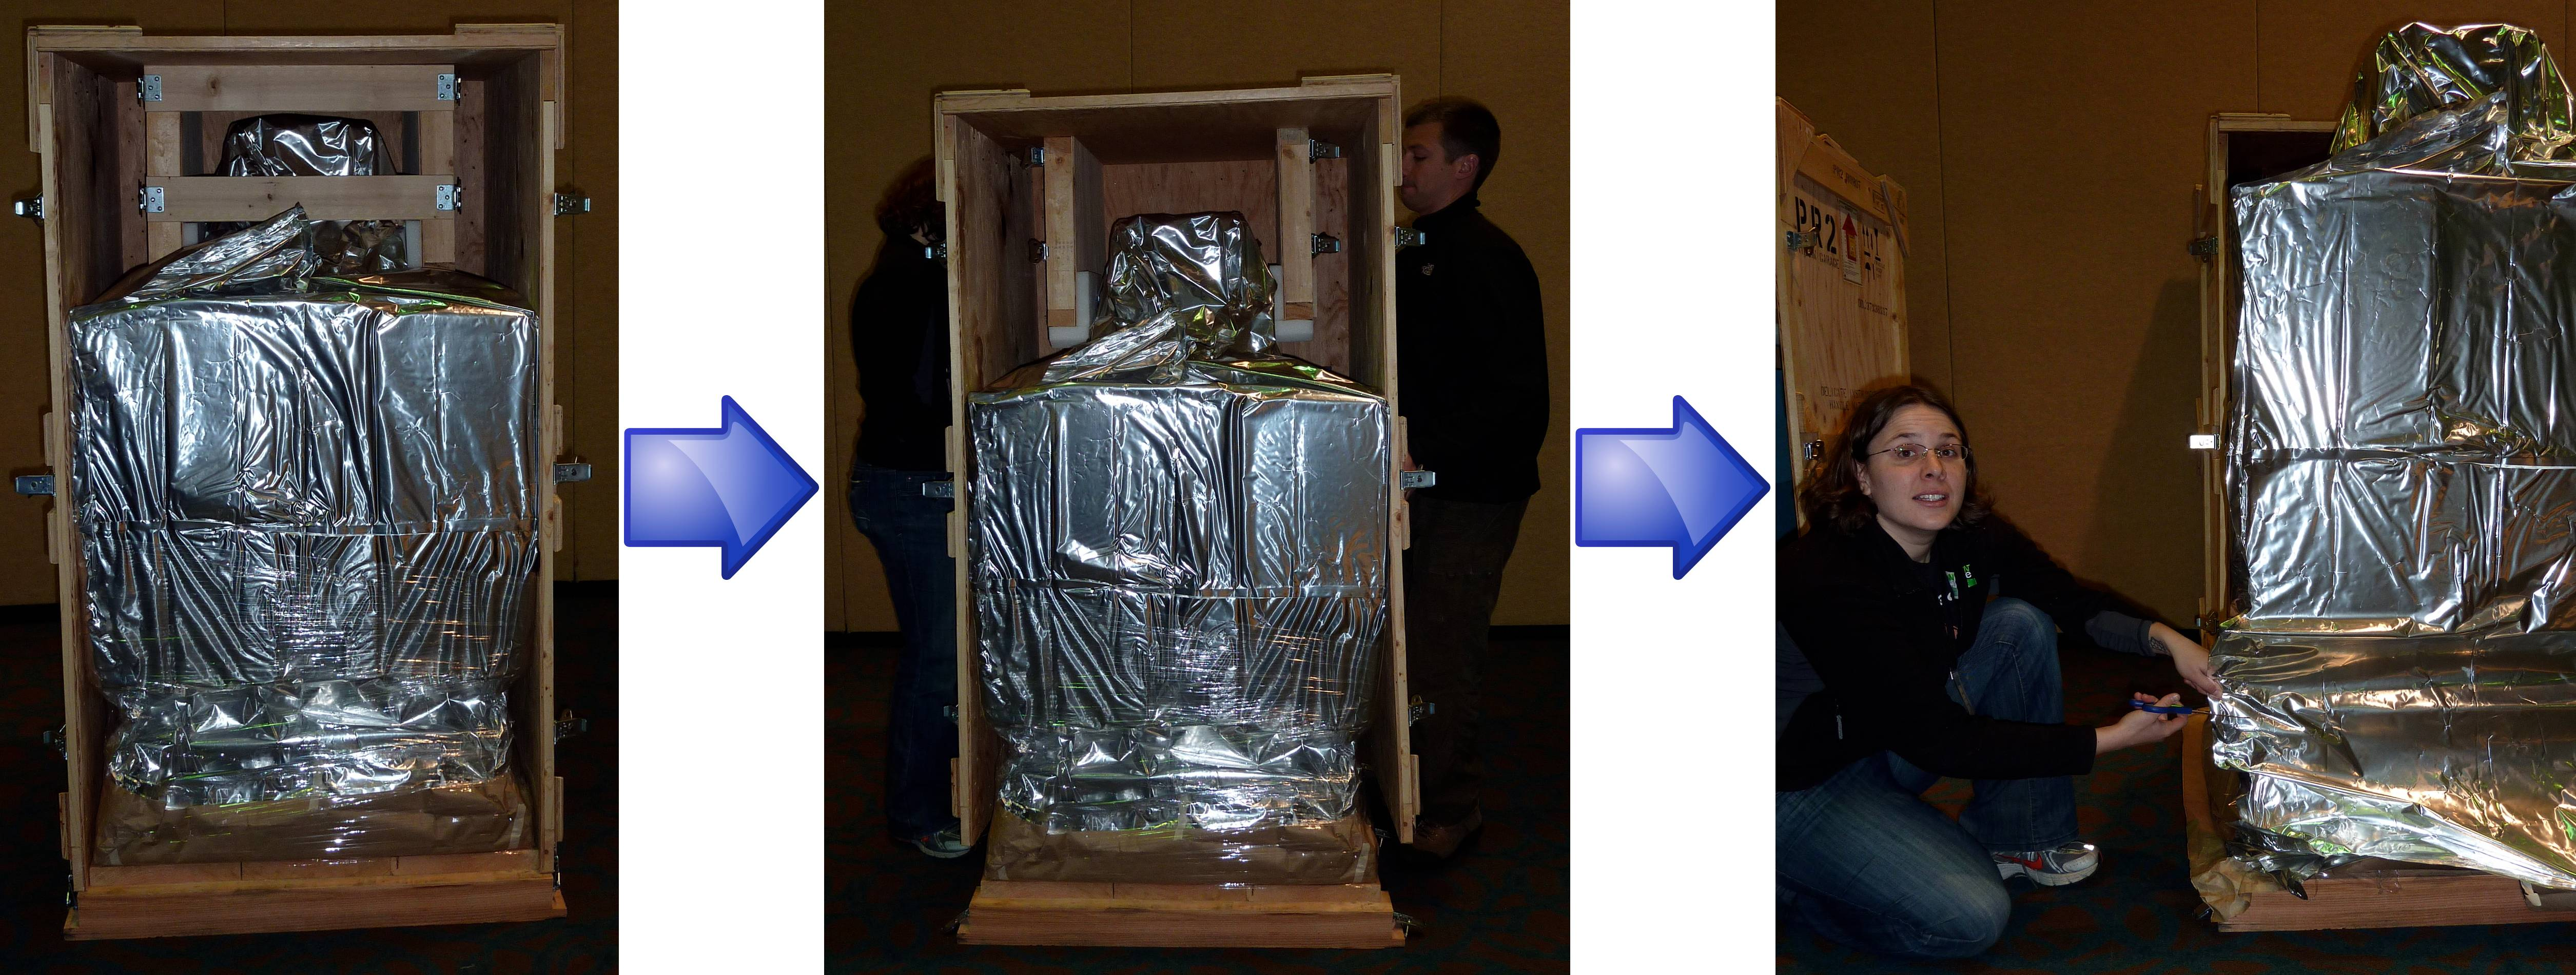
\includegraphics[width=\textwidth]{uncrate_lowres.jpg}
\caption{Steps for remvoing the crate.}
\label{fig:sealPR2}
\end{figure}

Now the top of the crate is completely unlatched. {\bf Verify that the two boards holding the head in place have been removed}, and then with two people grab opposite
sides of the crate and slowly walk the crate backwards off the crate
base. Remove all of the plastic wrapping and tape from around the foil vaccuum
wrapping. Once the wrapping is removed cut the foil wrapping about one foot up
from the seam all the way around the base of the robot, this will leave enough
material for repacking the robot if needed. Pull the foil wrapping off and
remove the dessicant bags from around the PR2, Figure~\ref{fig:unbagPR2}.

\begin{figure}[h]
\centering
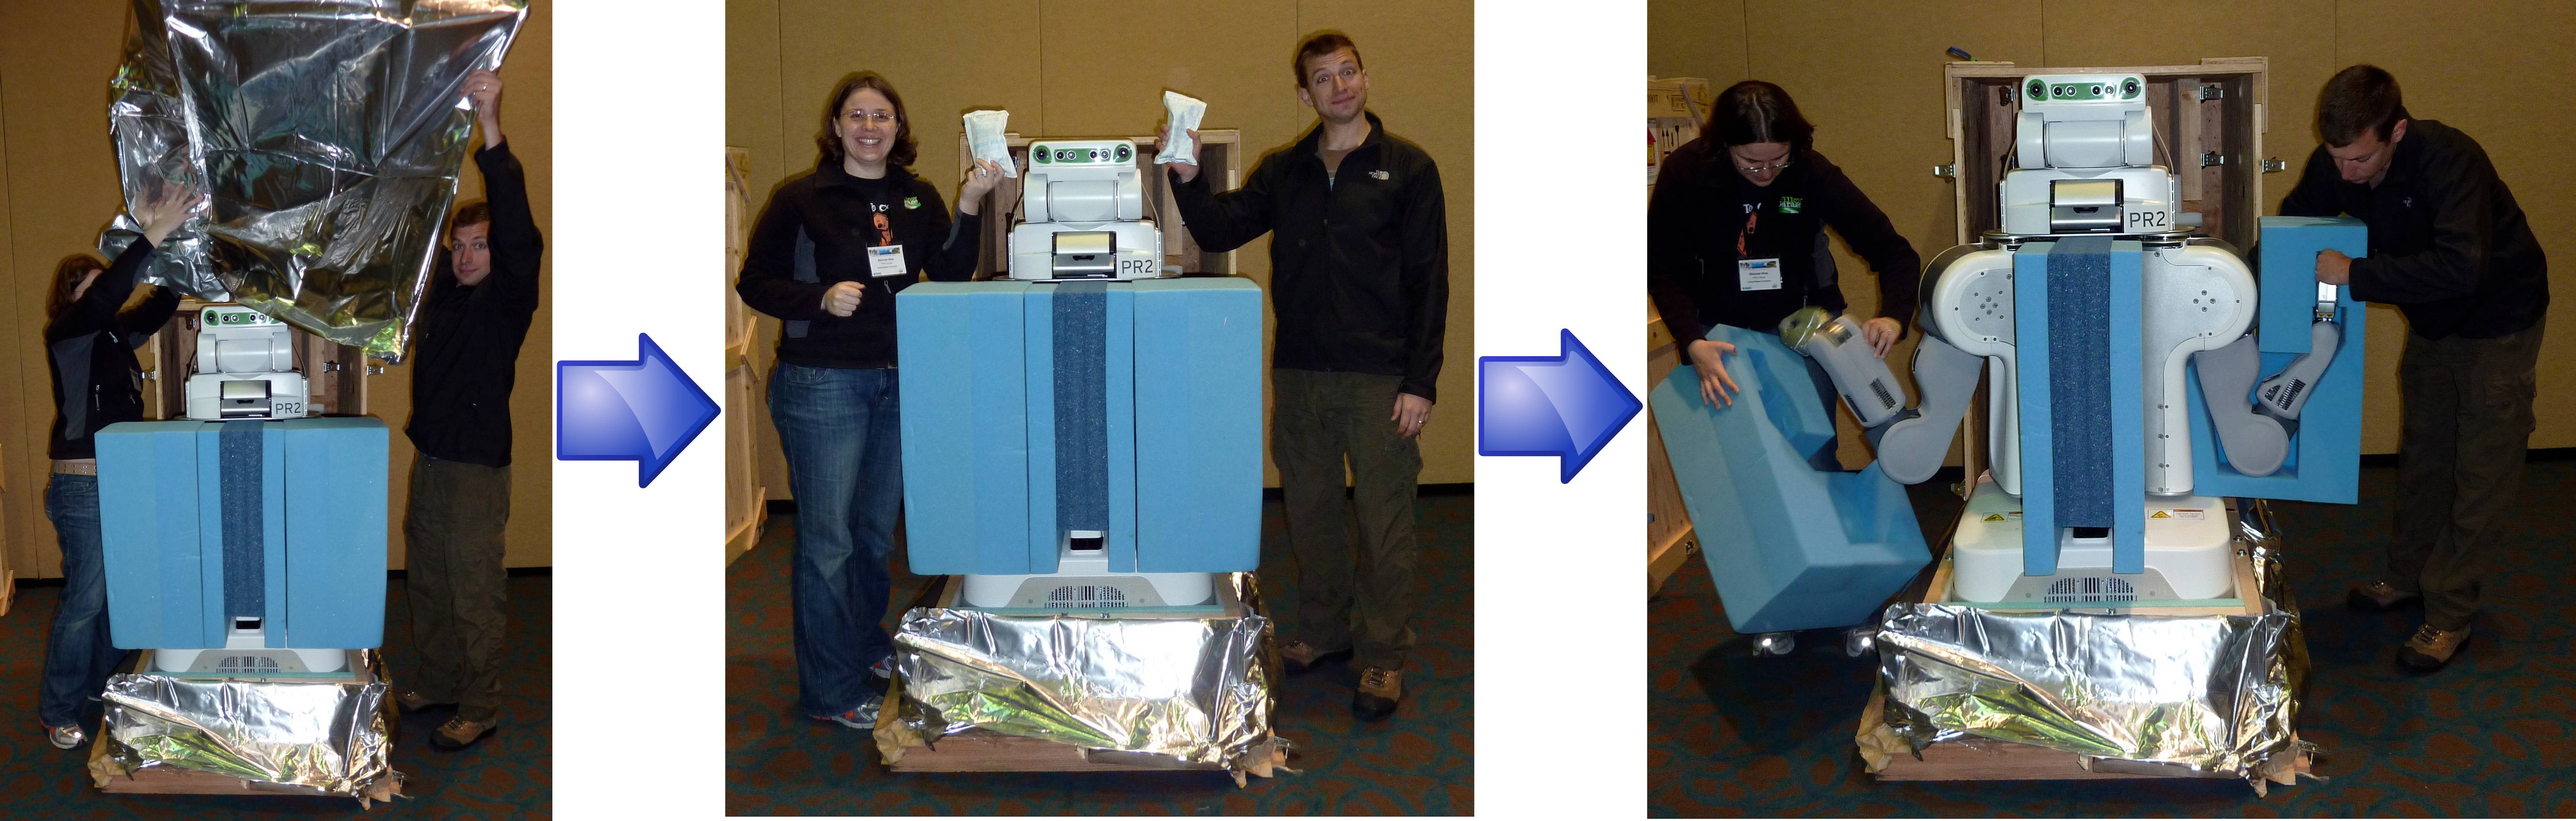
\includegraphics[width=\textwidth]{unbag_lowres.jpg}
\caption{Removing the foil wrapping, dessicant bags, and foam coverings.}
\label{fig:unbagPR2}
\end{figure}

Slide the foam coverings off of the arms and over the base laser, then remove
the bracing straps on each side of the head, Figure~\ref{fig:head_straps}, using
an 4mm allen wrench (this can be found in the robot toolkit). Place the straps and screws in a bag for later use when
repacking the PR2.

\begin{figure}[h]
\centering
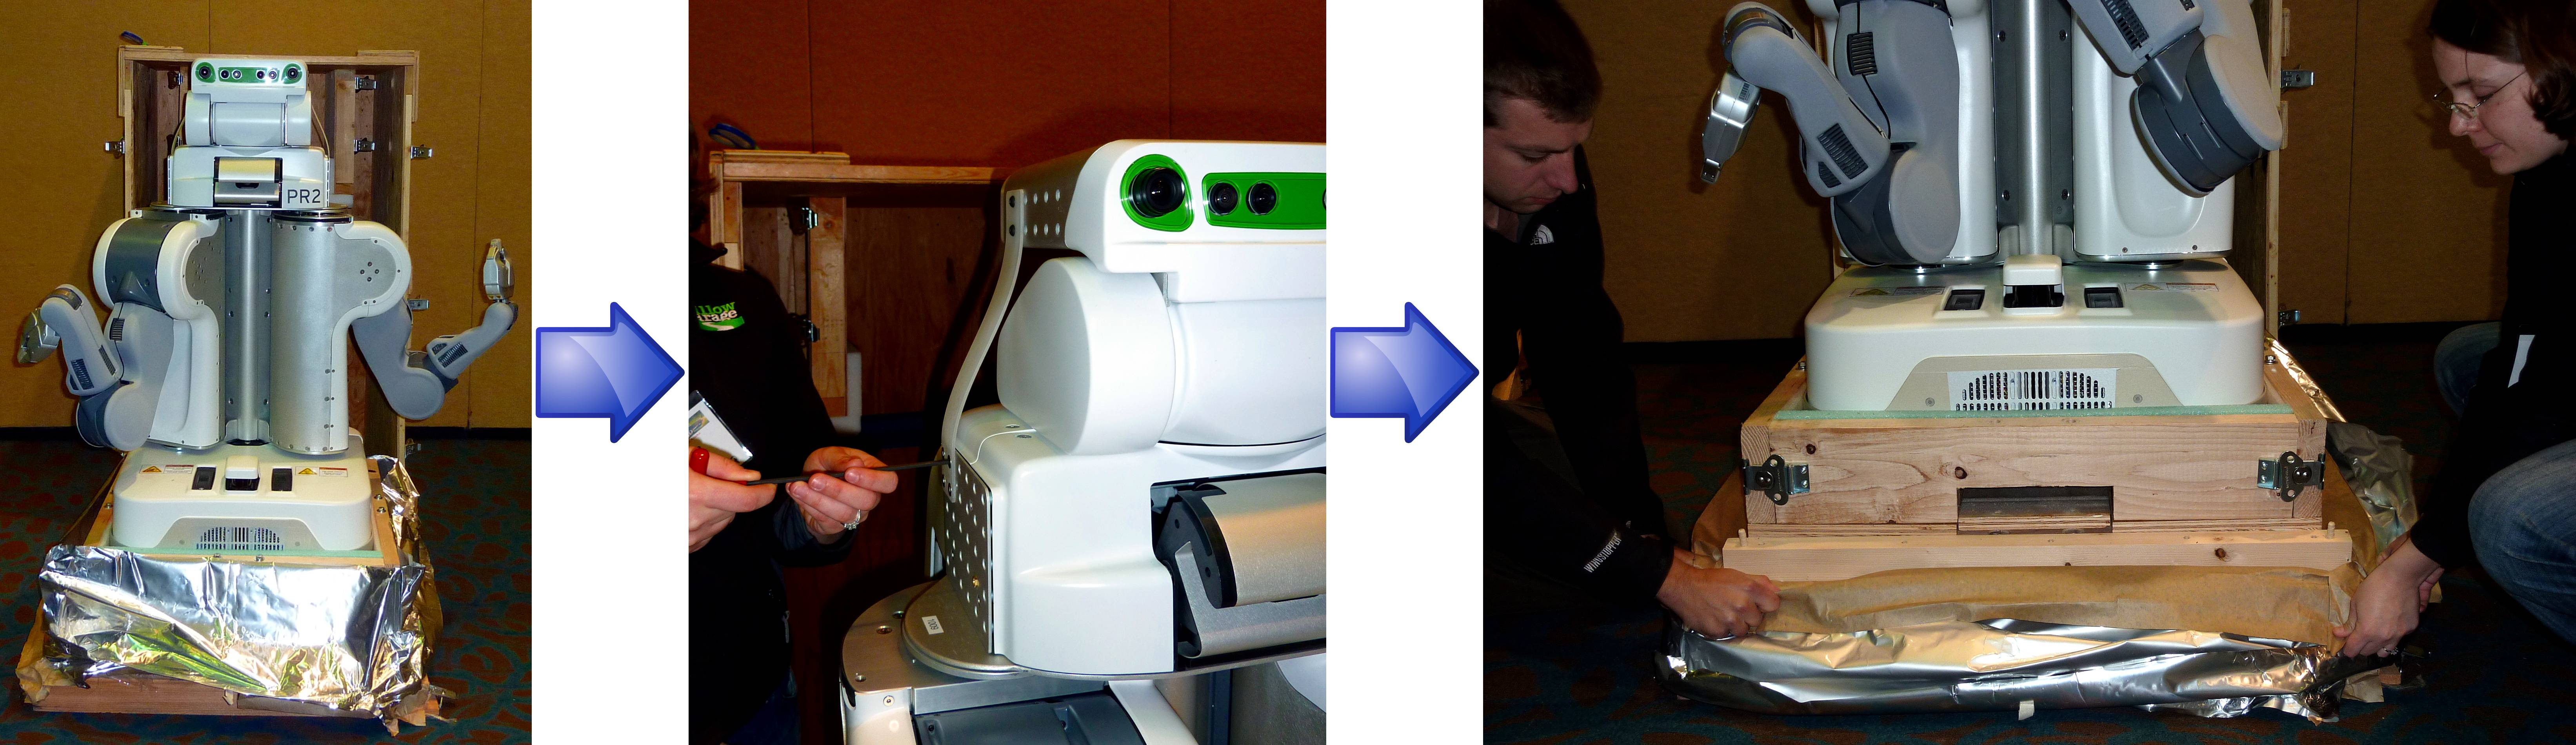
\includegraphics[width=\textwidth]{remove_head_brace_lowres.jpg}
\caption{Removing the head straps and pushing back packaging.}
\label{fig:head_straps}
\end{figure}

Push back the foil wrapping and other materials to reveal the platform in the
base of the crate. In the crate base beneath the PR2 platform is a support board
that must be removed {\bf before} unscrewing the bolts and lowering the platform, 
Figure~\ref{fig:unbolt}. Push the board from one side so that it protudes out the 
other side and pull it free. 

\begin{figure}[h]
\centering
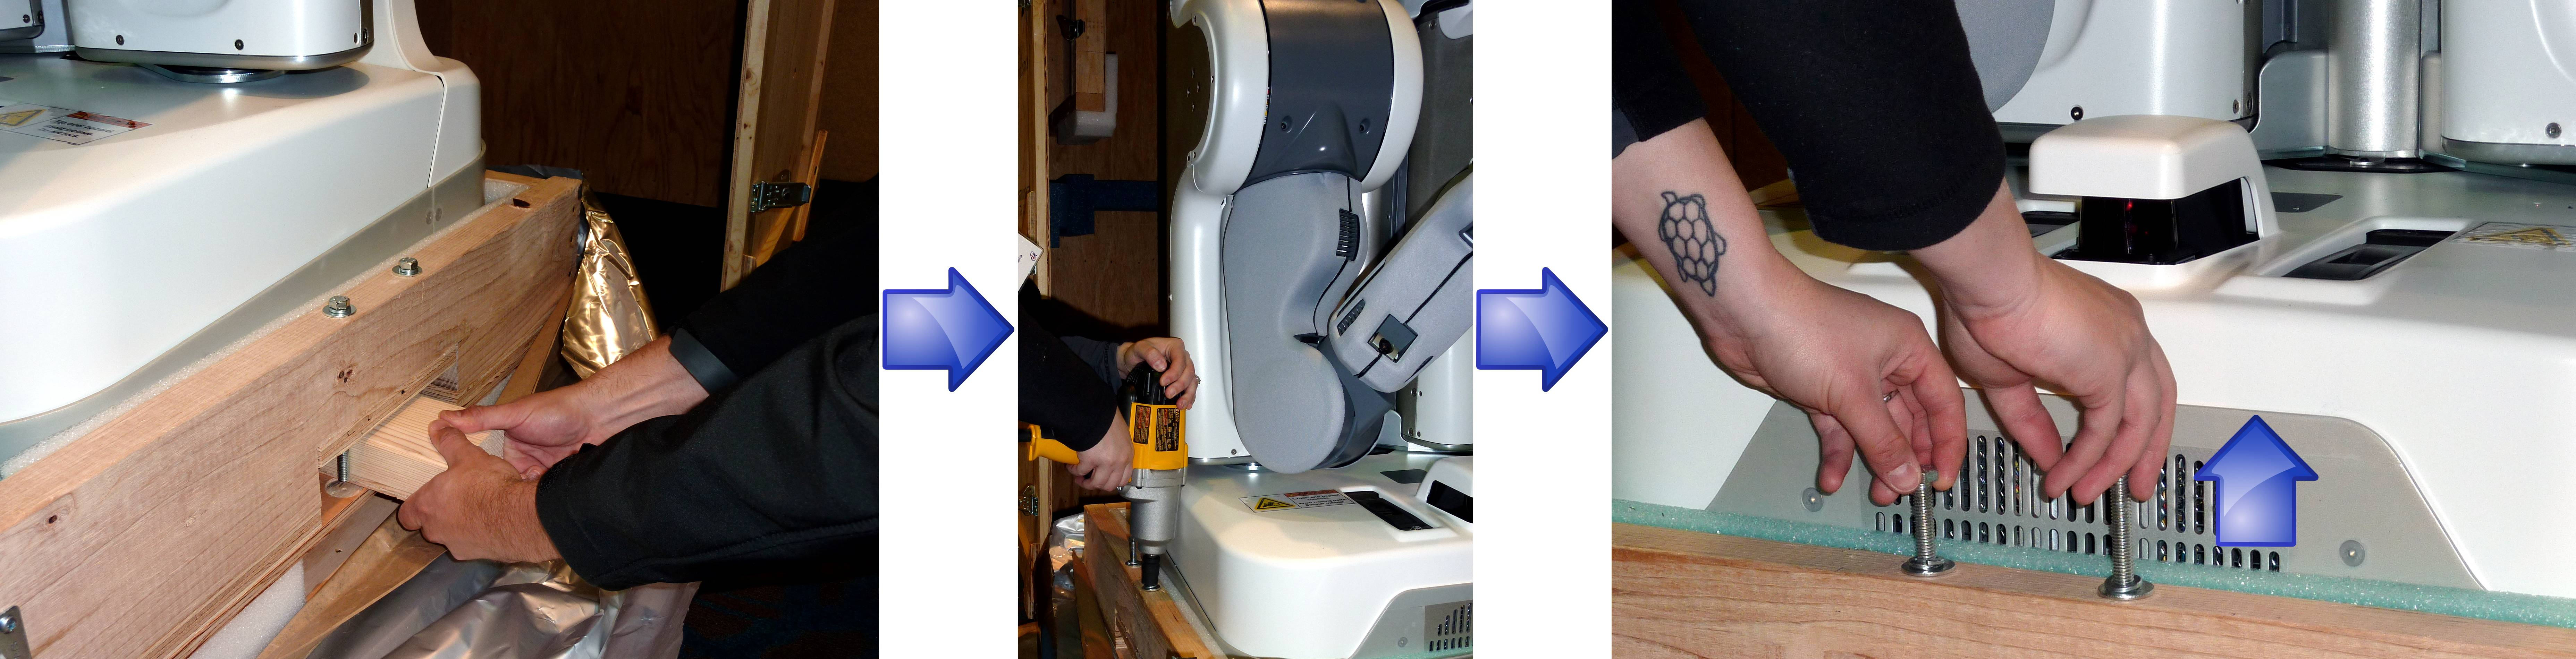
\includegraphics[width=\textwidth]{unbolt_lowres.jpg}
\caption{Removing support board, unscrewing and removing bolts.}
\label{fig:unbolt}
\end{figure}

Once the support board is free, use the drill to unscrew the bolts around
the crate base making sure that the two bolts in front of the robot come
completely out of the nuts. Unlatch the board in front of the PR2 base and set
it aside. With two people, take the panel labeled {\bf OPEN THIS PANEL FIRST} with
the label face up, so that the boards act as rails on the side of the panel, and lay the panel on the edge of the platform aligning the pegs
with the holes in the panel, as shown in Figure~\ref{fig:place_ramp}.

\begin{figure}[h]
\centering
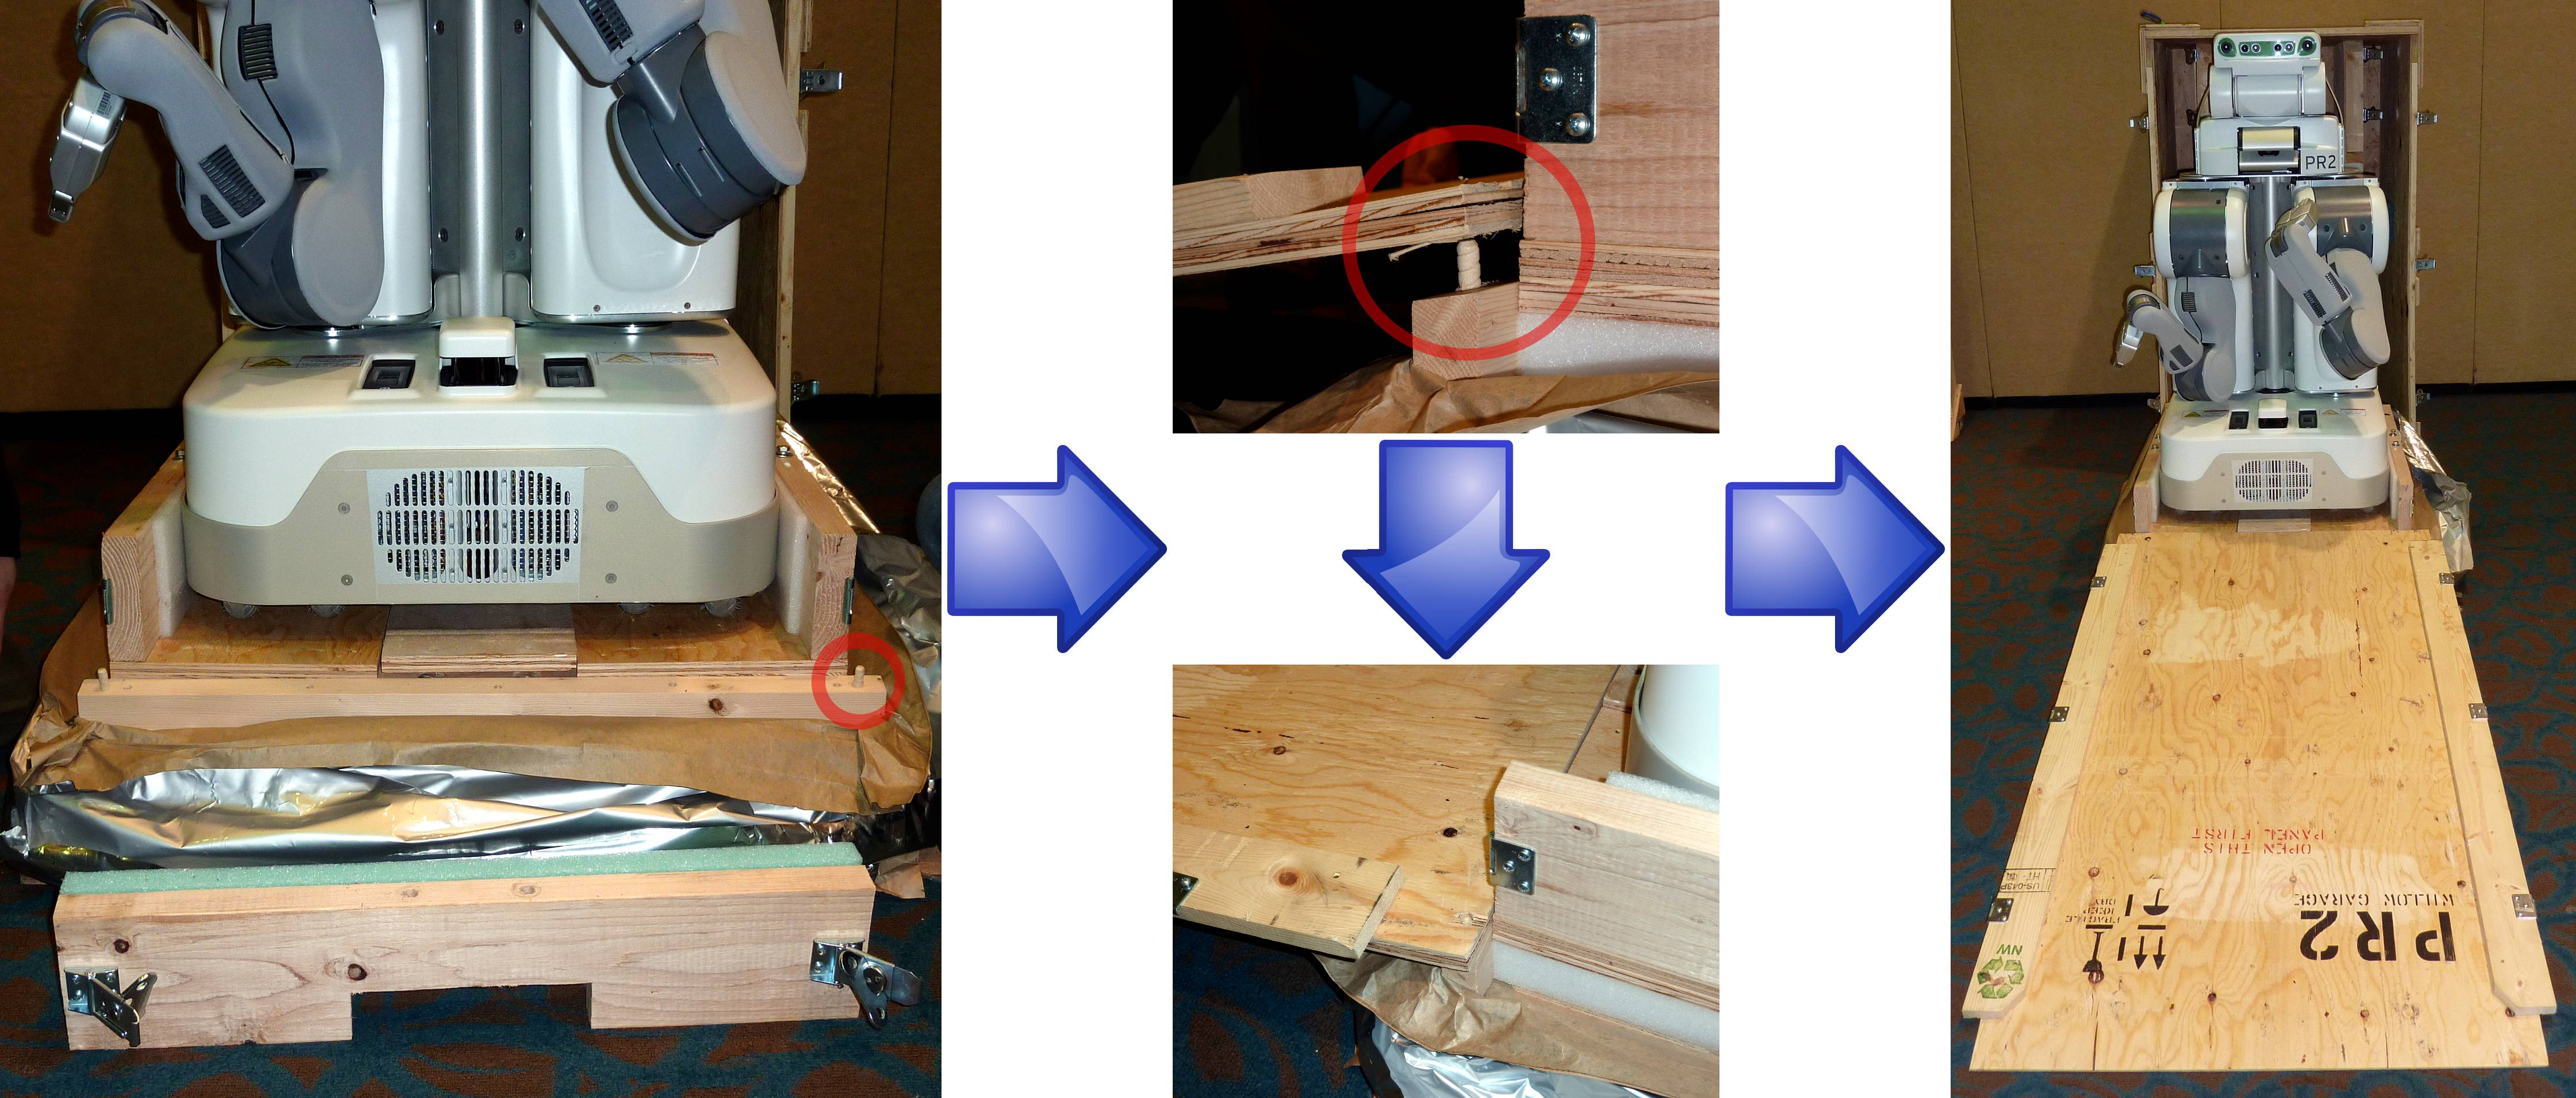
\includegraphics[width=\textwidth]{place_ramp_lowres.jpg}
\caption{Using the {\bf OPEN THIS PANEL FIRST} panel as a ramp.}
\label{fig:place_ramp}
\end{figure}

With the ramp in place, walk to the back of the robot and switch on the power switch
as shown in Figure~\ref{fig:switch_on}. Once the PR2 computers are booted connect 
to the PR2 wifi (PRXXXXLAN) using your wifi manager. The default password is ''willow''. 
After connecting to the wireless access point on the robot you can ssh into the robot 
as pr2admin with the default password of ''willow''. Once you are logged into the robot 
follow the directions outlined in Chapter 6 to drive the robot down the ramp. 

\begin{figure}[h]
\centering
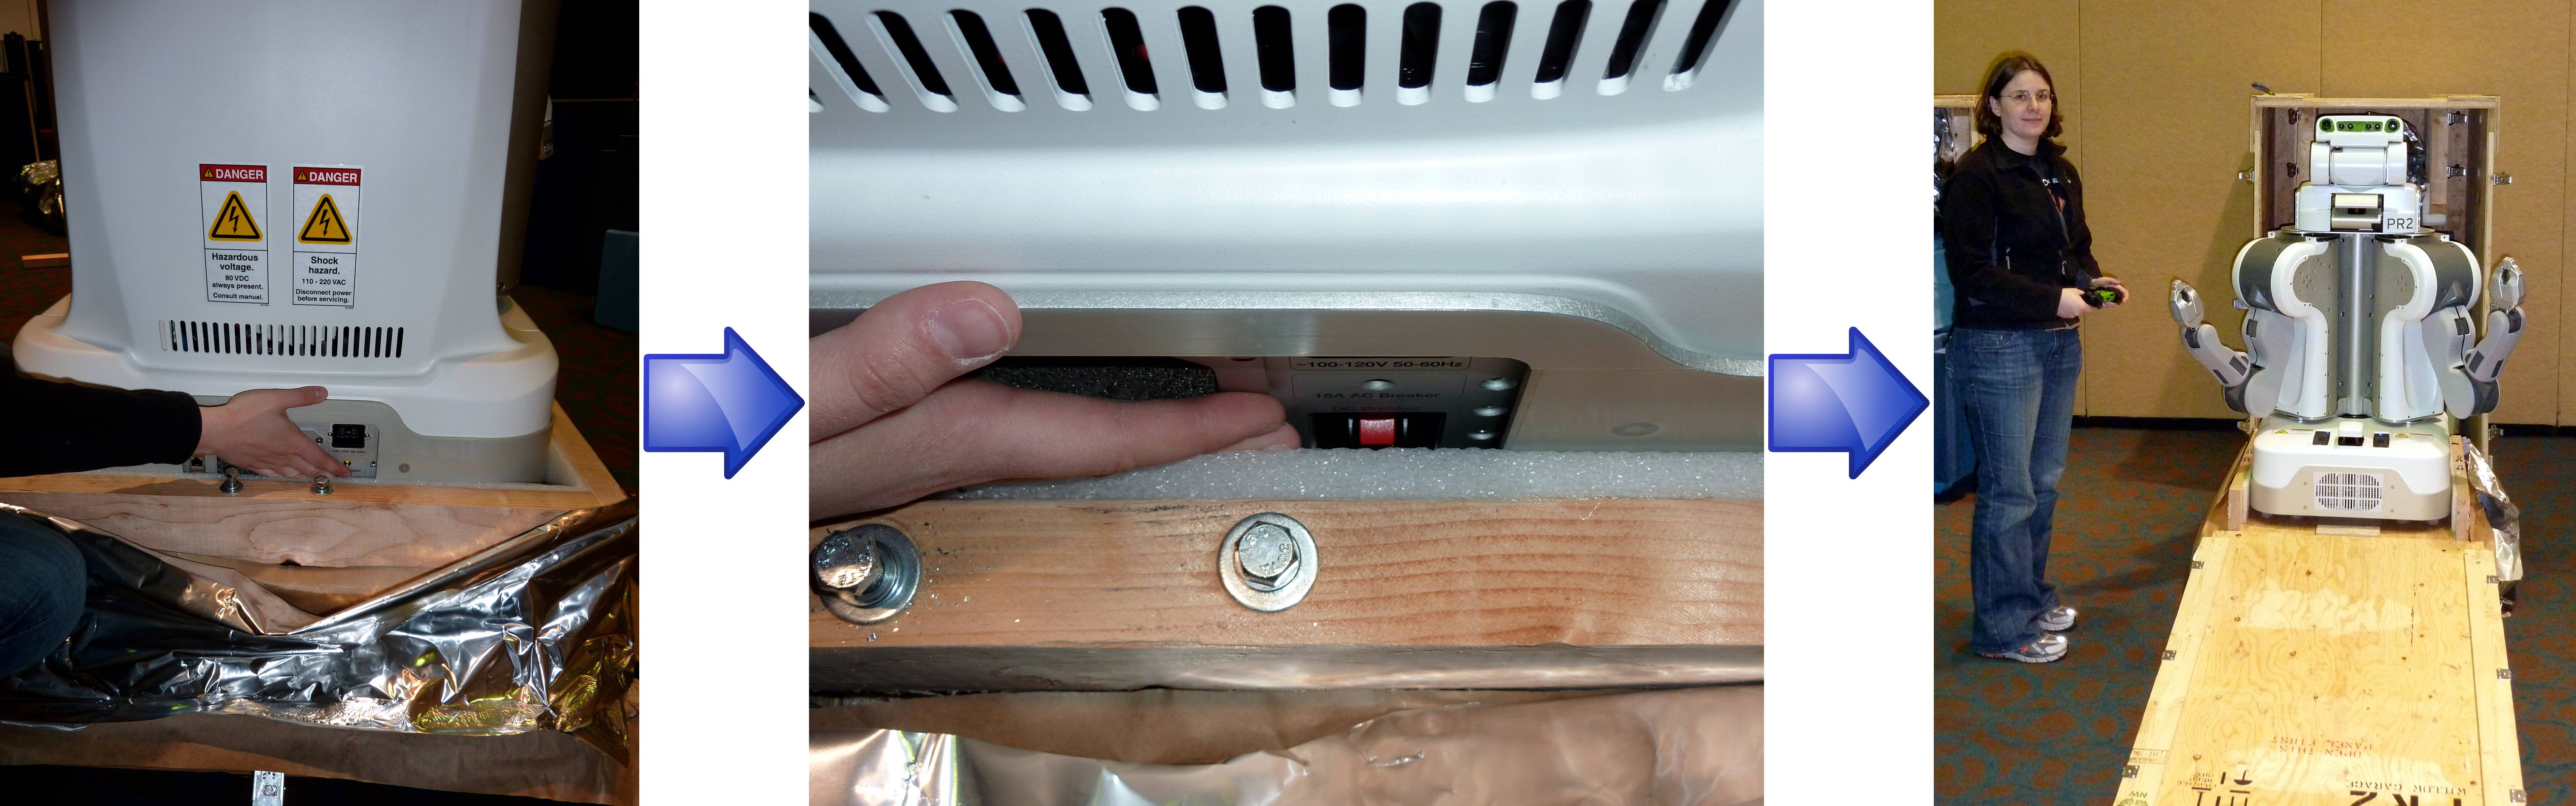
\includegraphics[width=\textwidth]{switch_on_lowres.jpg}
\caption{Switching on the PR2.}
\label{fig:switch_on}
\end{figure}

Please keep all shipping materials, including the crate, in storage.  They are useful for
moving the PR2 to another location, and will be required if you ever have to ship the PR2
back to Willow Garage for service.

